%---------------------------------------------------------------------------
% System use cases.
%
%---------------------------------------------------------------------------
\section{Use cases}
\label{sec:ch4_usecases}

In this section one may find usability analysis. This analysis is divided into 3 areas covering subsequent functional blocks: resources, measurements and visualizations. For each block, diagram in UML notation with additional description is provided. This approach is equal to the second level of detail in writing use cases, as proposed by A. Cockburn\cite{0201702258}. 

Because system isn't expected to work with sensitive information, there are no authorization mechanisms or access control management considered in this work. This also implies that in all diagrams, there is only one actor: User.

\subsection{Resources Management}
\label{subsec:resources_mgmnt}

Figure \ref{fig:usecase_resources} shows diagram depicting use cases related to resources management. This includes most generic actions like adding, removing, viewing state. Additionally application gives user ability to manage life cycle of specific resources (e.g. threads, processes) - user can pause, stop or resume previously paused item. What also should be mentioned, this diagram covers indirect actions that might be performed by user, like selecting which monitoring hub should be used to manage given resource, connecting to external monitoring hub, or even starting it.

\begin{figure}[ht]
\centering
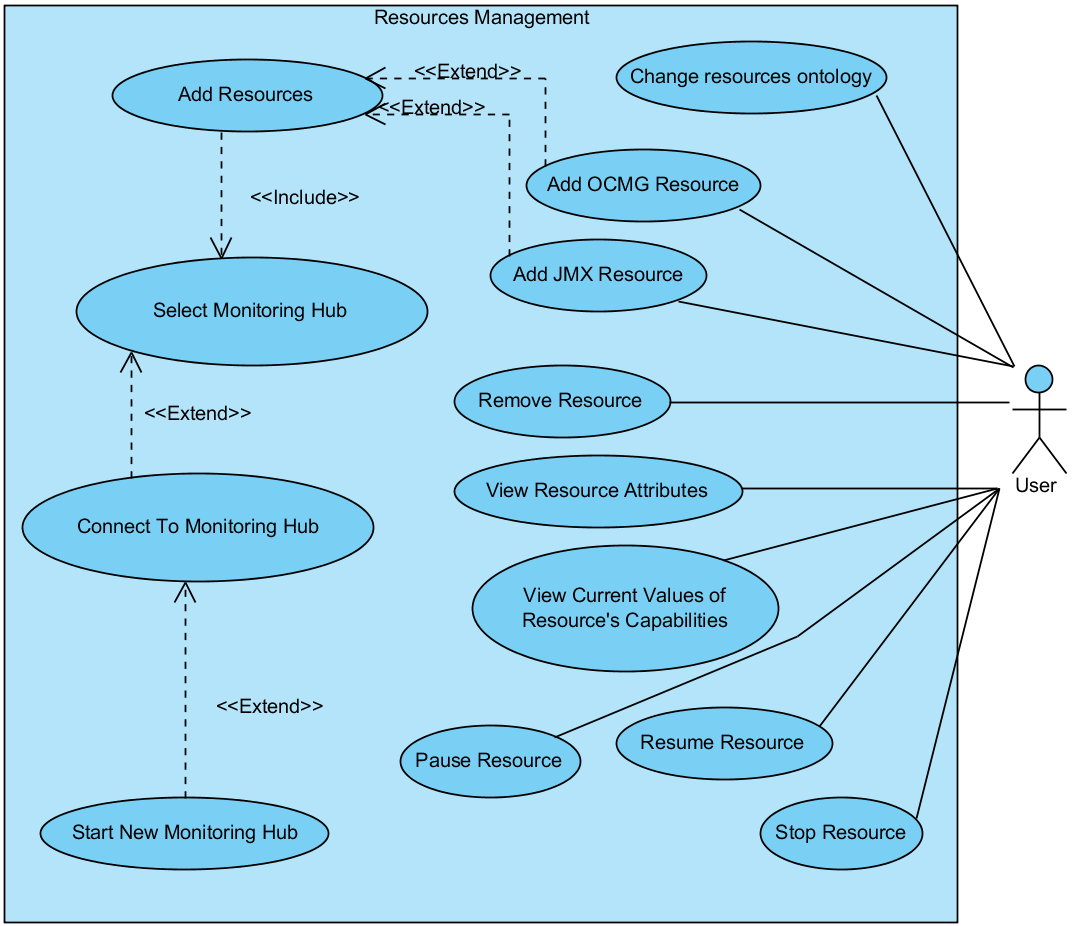
\includegraphics[width=0.8\textwidth]{resources}
\caption{Resources management use case diagram}
\label{fig:usecase_resources}
\end{figure}

Main use cases (actions performed by user directly to achieve his/hers aims):

\begin{itemize}
\item {\bf Add OCM-G Resource}~~~~~~~~~~~~~~~~~~~~~~~~~~~~~~~~~~~~~~~~~~~~~~~~~~~~~~~~\linebreak
Adding OCM-G resources. OCM-G resource is resources monitored using OCM-G monitoring system. This use case is specialization of more generic Add Resource use case. User should be able to select which application registered at Main SM to monitor. After selecting application, all its resources will be fetched and added to resource tree.

\item {\bf Add JMX Resource}~~~~~~~~~~~~~~~~~~~~~~~~~~~~~~~~~~~~~~~~~~~~~~~~~~~~~~~~\linebreak
Adding JMX resources. JMX resource is running JVM to which Monitoring Hub can connect using JMX protocol. While adding JMX resource, user can arrange them into labeled clusters and applications, and must specify URL that will be used by monitor to connect to JVM.

\item {\bf Remove Resource}~~~~~~~~~~~~~~~~~~~~~~~~~~~~~~~~~~~~~~~~~~~~~~~~~~~~~~~~\linebreak
Every added resource can be simply removed. All its measurements, and sub resources are removed as well.

\item {\bf View Resource Attributes} ~~~~~~~~~~~~~~~~~~~~~~~~~~~~~~~~~~~~~~~~~~~~~~~~~~~~~~~~\linebreak
By selecting previously added resource, user should be able to view given resource's static attributes. This is highly specific to resource type. For example, process resource may have attributes like executable path, command line attributes, etc.
\item {\bf View Current Values of Resource's
Capabilities}~~~~~~~~~~~~~~~~~~~~~~~~~~~~~~~~~~~~~~~~~~~~~~~~~~~~~~~~\linebreak
After selecting previously added resource, user can trigger fetch of all resource\rq{}s capabilities values and thus view snapshot of its state at current moment of time.

\item {\bf Pause Resource}~~~~~~~~~~~~~~~~~~~~~~~~~~~~~~~~~~~~~~~~~~~~~~~~~~~~~~~~\linebreak
User should be able to manage resource\rq{}s life cycle, if applicable. Specific resources like threads, processes, or nodes can be paused, which freezes processing made on given resource.

\item {\bf Resume Resource}~~~~~~~~~~~~~~~~~~~~~~~~~~~~~~~~~~~~~~~~~~~~~~~~~~~~~~~~\linebreak
As stated above, user can pause resource. User also should be able to resume previously paused resource.

\item {\bf Stop Resource}~~~~~~~~~~~~~~~~~~~~~~~~~~~~~~~~~~~~~~~~~~~~~~~~~~~~~~~~\linebreak
If resource allows it, user should be able to stop given resource totally. After stopping resource, no further calculations can be performed using given resource, and starting resource again is impossible. Stopping simply terminates resource.

\item {\bf Change Resources Ontology}~~~~~~~~~~~~~~~~~~~~~~~~~~~~~~~~~~~~~~~~~~~~~~~~~~~~~~~~\linebreak
User can change ontology that system internally uses to build resources tree. This change won\rq{}t be applied to currently discovered resource tree, but all newly added resources.

\end{itemize}


Indirect use cases (actions performed by user indirectly to help perform direct actions):

\begin{itemize}

\item {\bf Add Resource}~~~~~~~~~~~~~~~~~~~~~~~~~~~~~~~~~~~~~~~~~~~~~~~~~~~~~~~~\linebreak
Generalization of Add JMX Resource and Add OCM-G Resource use cases. It was extracted to ease modeling of functionalities provided by those use cases, like selecting monitoring hub.

\item {\bf Select Monitoring Hub}~~~~~~~~~~~~~~~~~~~~~~~~~~~~~~~~~~~~~~~~~~~~~~~~~~~~~~~~\linebreak
To be able to add resource, user has to select monitoring hub that will be responsible for managing resources and gathering data related to them.

\item {\bf Connect to Monitoring Hub}~~~~~~~~~~~~~~~~~~~~~~~~~~~~~~~~~~~~~~~~~~~~~~~~~~~~~~~~\linebreak
User should be able, to connect to manually started, potentially remote, monitoring hub, prior to selecting one.

\item {\bf Start New Monitoring Hub}~~~~~~~~~~~~~~~~~~~~~~~~~~~~~~~~~~~~~~~~~~~~~~~~~~~~~~~~\linebreak
User should be able to start new, potentially remote monitoring hub, prior to connecting and using it.

\end{itemize}

\subsection{Measurements Management}
\label{subsec:measurement_mgmnt}

\begin{figure}[ht]
\centering
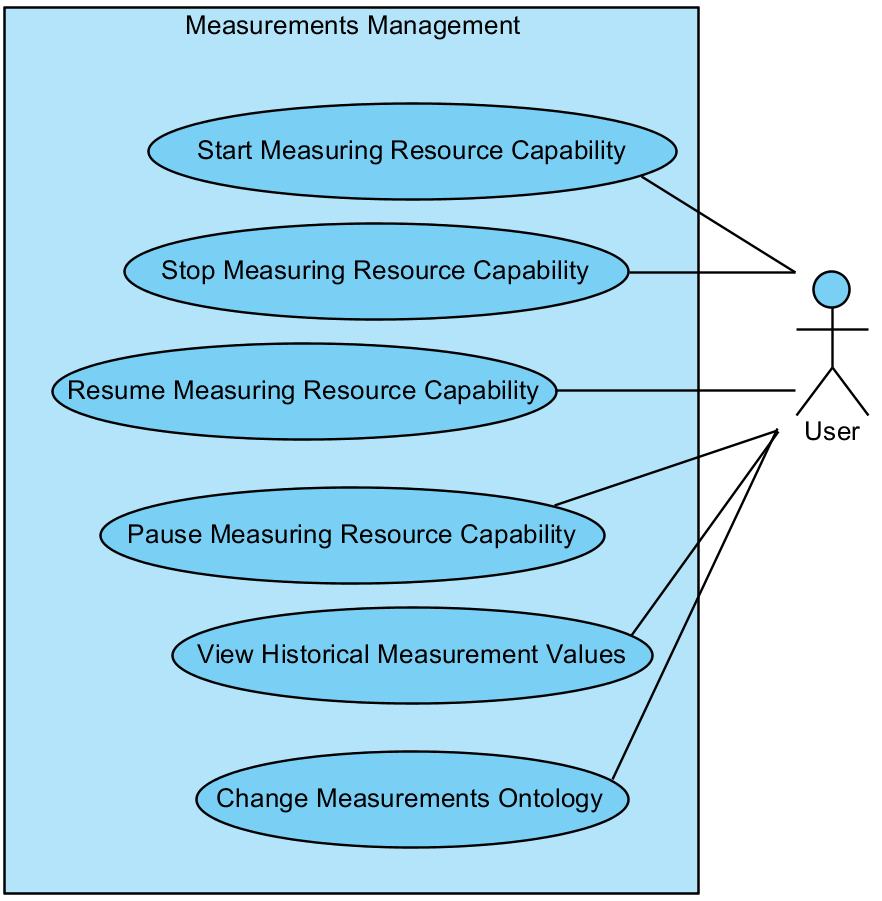
\includegraphics[width=0.5\textwidth]{Measurements}
\caption{Measurements management use case diagram}
\label{fig:usecases_measurements}
\end{figure}

Figure~\ref{fig:usecases_measurements} shows use cases related to measurement management. Measurement functionalities are a bit less complex then resources management. User is able to create and start (which is merged into one action), stop, pause, resume measuring values of given capabilities. Additionally user can view all historical values, of given measurement.

\subsection{Visualizations Management}
\label{subsec:visualizations_mgmnt}

Figure~\ref{fig:usecases_visualisations} depicts diagram of use cases related to management of measurement visualizations. Visualizations functional block contains following actions:

\begin{itemize}

\item {\bf Add Visualization}~~~~~~~~~~~~~~~~~~~~~~~~~~~~~~~~~~~~~~~~~~~~~~~~~~~~~~~~\linebreak
User can add new, empty (without any measurements attached) visualization. It is basic first step that needs to be done to visualize measurements.

\item {\bf Add Measurement to Visualization}~~~~~~~~~~~~~~~~~~~~~~~~~~~~~~~~~~~~~~~~~~~~~~~~~~~~~~~~\linebreak
After creating new visualization, user can add measurements, which makes visualization facility fully functional.

\item {\bf View Visualization}~~~~~~~~~~~~~~~~~~~~~~~~~~~~~~~~~~~~~~~~~~~~~~~~~~~~~~~~\linebreak
It\rq{}s most obvious use case - after creating visualization, attaching measurements user can view results of measurements using provided plots.

\item {\bf Remove Measurement from Visualization}~~~~~~~~~~~~~~~~~~~~~~~~~~~~~~~~~~~~~~~~~~~~~~~~~~~~~~~~\linebreak
User should be able to remove previously attached measurements from given visualization.

\item {\bf Remove Visualization}~~~~~~~~~~~~~~~~~~~~~~~~~~~~~~~~~~~~~~~~~~~~~~~~~~~~~~~~\linebreak
When given visualization isn't needed by user anymore, it can be simply removed from application.

\item {\bf Edit Visualization Display Options}~~~~~~~~~~~~~~~~~~~~~~~~~~~~~~~~~~~~~~~~~~~~~~~~~~~~~~~~\linebreak
User should be able to have additional level of control over visualizations. Managing plot type allows it - user should be able to change display type of already created visualization.

\item {\bf Change Measurements Ontology}~~~~~~~~~~~~~~~~~~~~~~~~~~~~~~~~~~~~~~~~~~~~~~~~~~~~~~~~\linebreak
User can change the ontology that defines capabilities that given resource has.

\end{itemize}

\begin{figure}[ht]
\centering
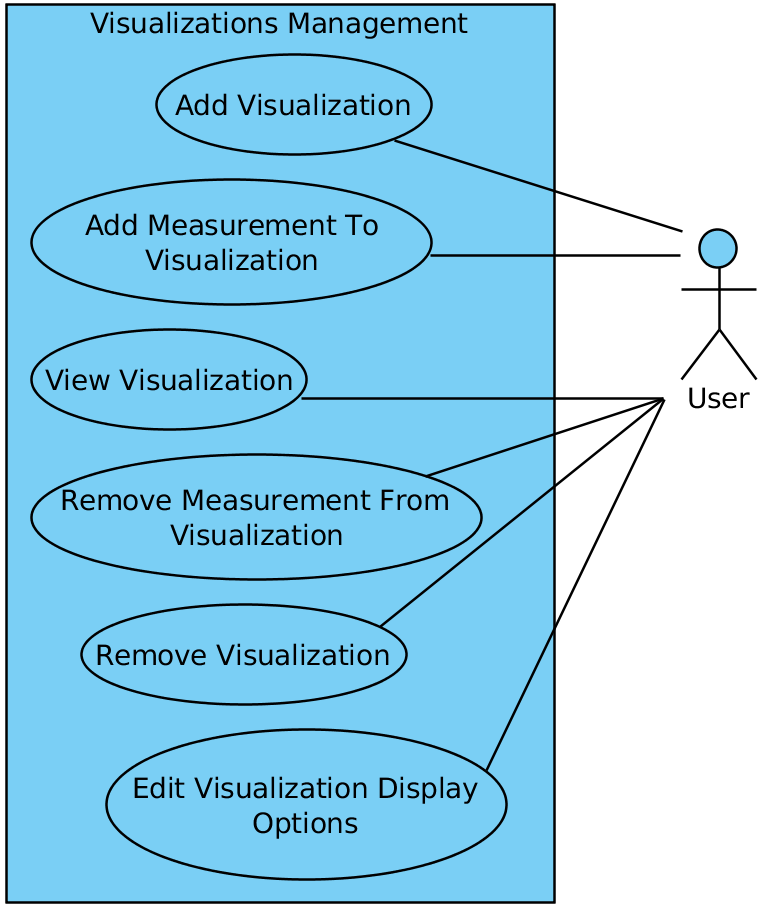
\includegraphics[width=0.4\textwidth]{Visualizations}
\caption{Visualizations management use case diagram}
\label{fig:usecases_visualisations}
\end{figure}
